\chapter{Примерна архитектура за реактивни приложения. Конкретни средства за реализация}
\label{ch:reactive-architecture}

Реактивните приложения и тяхната ориентираност около съобщения ни предоставят изключително голяма гъвкавост относно тяхната архитектурата. Слабо свързаните компоненти ни позволяват да изграждаме и оптимизираме подсистеми, съобразени с изискванията на отделните компоненти и начинът, по който те ще бъдат използвани. В тази глава ще предложим вариант за обща архитектура на не големи до средно големи реактивни приложения, които ще разгледаме заедно с конкретни реализации, съобразени с реактивните инструменти от предишната глава, които ще използваме за реализирането на конкретно приложение.

\section{Общ поглед}

\begin{figure}
  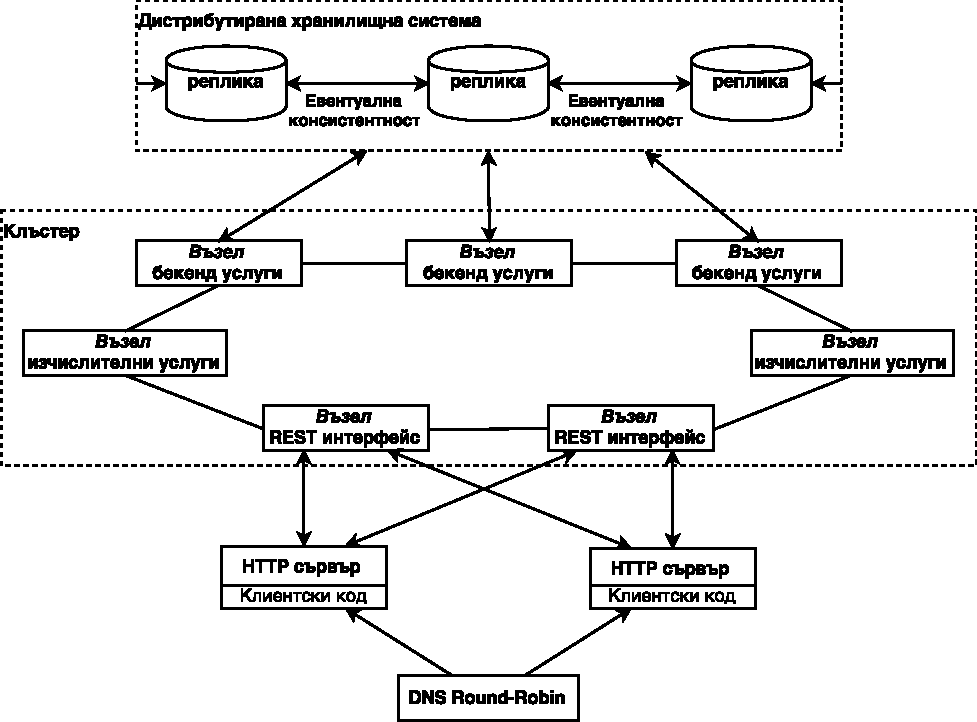
\includegraphics[width=\textwidth]{images/architecture.pdf}
  \caption{Примерна реактивна архитектура}
  \label{fig:reactive-architecture}
\end{figure}

\shortlabeledref{Фигура}{fig:reactive-architecture} представя общ поглед на архитектурата, която предлагаме в тази глава. Състои се от следните елементи:

\begin{itemize*}
  \item \emph{Клиентско приложение и клиентски HTTP сървър} — сервират клиентския код и осигуряват фасада към различни интерфейси.
  
  \item \emph{Клъстер от услуги} — съвкупност от възли, осигуряващи различни услуги като част от приложението. Възлите могат да се делят на различни типове, предлагащи различни типове услуги. От всеки тип може да имаме различен брой възли, в зависимост от нуждите на приложението. Тук ще разгледаме следните типове:
  
  \begin{itemize*}
    \item \emph{интерфейсни възли} — осигуряват връзка с услугите на приложението и различни интерфейсни функционалности;
    
    \item \emph{изчислителни възли} — възли, предназначени за тежки изчисления, натоварващи процесорите;
    
    \item \emph{бекенд възли} — общи възли, поемащи останалите услуги на приложението, включително управление на данните.
  \end{itemize*}
  
  \item \emph{Дистрибутирана хранилищна система} — базите от данни на приложението, осигуряващи дистрибутираност и репликация чрез евентуална консистентност.
\end{itemize*}

В следващите секции ще разгледаме всеки от елементите по-подробно, както и подходи, свързани с тяхното използване.

\section{Клиентско приложение и клиентски HTTP сървър}

Често клиентската част на реактивните приложения е от типа на т.~нар. едностранични приложения (\englishterm{single page application}). Това са статични файлове, съдържащи цялата логика за потребителския интерфейс, зареждащи се наведнъж. Клиентското приложение работи самостоятелно и напълно независимо от останалите услуги на системата. Поради поточната природа на реактивните приложения често те си пасват най-добре с клиентски приложения, базирани на \englishterm{dataflow} модел, абстрахиращ силно императивната природа на DOM модела на уеб страниците. Затова може да се използва например FRP-базирани (функционално реактивно програмиране) библиотеки в комбинация с т.~нар. „виртуален DOM“, позволяващи функционален начин на разпространение на данните и изменение DOM дървото. Други популярни подходи са използването на React.js библиотеката, също предоставяща функционален виртуален DOM и лека форма на реактивен поток, или Angular,js библиотеката, предоставяща императивен \englishterm{dataflow}, но с декларативен модел. Различните подходи биха могли да се комбинрат заедно.

Важен фактор е, че клиентските приложения трябва да са отзивчиви когато сървърните части на приложението не работят пълноценно или са силно натоварени. В такива случаи те трябва да уведомяват потребителите по подходящ начин.

Клиентското приложение се сервира от HTTP сървър за статични файлове. Допълнително сървърът трябва да осигурява фасада към същинските услуги на приложението, проксифицирайки определени пътища към тях и осигурявайки баланс на натоварването. Цялата комуникация ще минава през тях, затова тези сървъри трябва да могат да поддържат голям брой потребители. Именно най-подходящи са сървърите, базирани на \emph{реактор или проактор} шаблоните. Такъв сървър е Nginx, който ще използваме в реализацията в следващата глава. Той е оптимизиран специално за тези две функции за сервиране на статични файлове и проксифициране и балансиране към други услуги. Базира се на модел чрез множество реактори.

Поради еластичността на интерфейсните възли клиентските сървъри трябва да следят техния брой и местоположение. Nginx предоставя разширение, което динамично ги извлича от база от данни, или алтернативно позволява лесно презареждане на настройките си по време на изпълнение.

Поради това че в интерфейсните възли често се извършва кеширане, е добре едни и същи клиенти да бъдат проксифицирани към едни и същи възли, което може да се подсигури с HTTP бисквитка.

Броят на клиентските HTTP сървъри обикновено е по-рядко променящ се, тъй като единствено предават данни без да извършват обработка. Към тях обаче също трябва да бъде извършвано балансиране. Това става чрез т.~нар. \englishterm{DNS Round-Robin} \cite{rfc1794}. При него всеки сървър стои на различен IP адрес, а домейн името на приложението се свързва с всеки от тях, като DNS сървърът върти тяхната подредба. Благодарение на това различните клиенти балансирано използват различни сървъри.

\section{Клъстер от услуги}

Това е съвкупност от възли, осигуряващи същинските услуги на приложението. Възлите могат да комуникират помежду си, всеки с всеки. За реализация всеки възел ще представлява различна актьорска система. За свързване на актьорските системи ще използваме разширението за клъстери на библиотеката Akka.

Разширението предоставя устойчива реализация, която издържа на временни частични грешки и деления в мрежата. За следене на състоянието на мрежата и възлите използва специален \englishterm{gossip} протокол, при който списъкът с активните възли се разпространява постоянно сред всички участници. Начинът на работа се базира на дистрибутираната база от данни Дайнамо на Амазон и е описан в документацията на Akka, както и в \cite{deCandia2007Dynami}.

Протоколът позволява откриване на частични деления в мрежата и недостижими възли. Характерно свойство е, че когато това се случи към клъстера не могат да се присъединят нови възли, докато мрежата не се възстанови или докато недостижимите възли не бъдат премахнати, което става след конфигурируем таймаут. Премахнатите възли не могат да се присъединят отново към клъстера без да бъдат рестартирани. Всичко това може да доведе до съществуване на няколко работещи по-малки клъстера, тъй като всеки от тях ще открил другите възли като неналични. Това може да е проблем при някои приложения и затова трябва да се конфигурира в зависимост от желаното поведение. Akka оставя системния администратор да вземе коригиращи действия при дълго продължили мрежови деления, тъй като софтуерно не може да бъде гарантирана тяхната поправка.

Към клъстера могат да се добавят и от него премахват възли във всеки един момент, в който липсват мрежови деления. Така може да бъде осигурена еластичност сравнително лесно. За целта възелът, който иска да се присъедини, трябва да познава някой от членовете на клъстера. Поради тази причина няколко от сигурните възли се посочват в конфигурацията като възли от клъстера, наречени още \englishterm{seeds}. Освен тях обаче всеки друг възел не е необходимо да бъде предварително зададен.

Всеки възел в клъстера може да има собствена логика и обикновено бива маркиран с определена роля.

\section{Домейн модел и модел на данните}

Изключително важна част от архитектурата, която не е отразена на общия поглед от \shortlabeledref{фигура}{fig:reactive-architecture}, са моделирането на домейн обектите и тяхната персистентност. Тук ще разгледаме стандартен подход за дистрибутирани системи.

\subsection{Разделение на отговорността за командите от тази за заявките}

Шаблонът CQRS \cite{young2010CQRS}, който споменахме още в \shortlabeledref{глава}{ch:reactive-programming-principles}, предлага прости принципи, които се оказват доста полезни за дистрибутираните системи. Един от основните проблеми при използването на CRUD операции и общ модел за четене и запис, което имаме при стандартните архитектури, е че те дават само определен поглед над данните. CRUD дава единствено крайния резултат — промяна в определени полета или изтриване на запис, но не и как е била изчислена промяната и при какво действие е била извършена. От своя страна ефективната трансформация или агрегация на модела при някои заявки е трудна, а понякога и невъзможна, ако причината за промяната е била изгубена.

CQRS изисква друг подход. При него боравенето със данни се разделя на команди, които извършват само промени, и заявки, които единствено връщат резултати, без да променят състояние. При CQRS за двете отговарят напълно независими компоненти. Командите изразяват точно това, което потребителят е извършил като действие. Затова този шаблон пасва силно с принципите на \englishterm{Domain-Driven Design} \cite{evans2003DDD}. Командите минават през отделен интерфейс, стигат до съответния компонент, който ги валидира и при успех ги записва в своето хранилище и потвърждава записа на клиента. Аналогично четенето на данни минава от друг интерфейс до компонента, отговорен за това. Той може да вземе данните от хранилището на командите. По-интересно е обаче е това, че заявките могат да използват различно хранилище и различен модел на данните, специално оптимизиран за тях. Това може да се реализира като специален компонент следи хранилището на командния компонент, или пък самият команден компонент генерира събитие при промяна с това каква команда е била извършена. Така множество интересуващи се модели за заявки могат да се абонират за събитията, да обновяват своето състояние, реагирайки на реално извършената команда, и да го съхранят в подходящ формат, евентуално дори в различна база от данни, оптимизирана за него. Ако събитията се генерират асинхронно това може да доведе до евентуална консистентност, което е подходящо за дистрибутирани системи. С този подход също така данните могат да бъдат репликирани на отделечени системи.

\shortlabeledref{Фигура}{fig:cqrs-in-action} показва шаблона в действие. При наличие на различни модели за заявки бихме имали конкретен команден наблюдател за всеки един.

\begin{figure}
  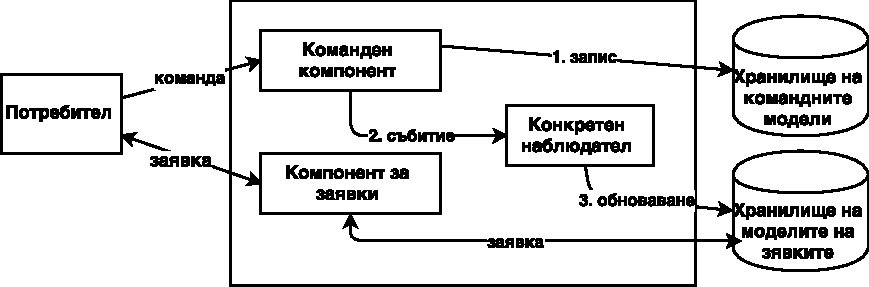
\includegraphics[width=\textwidth]{images/cqrs.pdf}
  \caption{Интеракции при CQRS}
  \label{fig:cqrs-in-action}
\end{figure}

\subsection{\englishterm{Event sourcing}}

Допълнение към CQRS може да бъде т.~нар. \emph{event sourcing}. При него вместо текущото състояние на даден агрегат (\cite{evans2003DDD}) в хранилището се поддържа журнал от всички събития, генерирани върху него. Към този журнал единствено се прилепят нови събития, без да се трият стари, което е бърза операция. Ако всички те бъдат приложени се получава текущото състояние на агрегата. Този подход е функционален по природа, тъй като избягва изменяемо състояние, и отново е приложим за дистрибутирани и конкурентни системи, например за евентуално постигане на консистентност когато агрегата е променян от различни източници. Ако се пази само текущото състояние това би било доста по трудно. За оптимизация е възможно периодично да бъде правена снимка на агрегата, като състоянието бива възстановявано от нея и всички последващи събития. \englishterm{Event sourcing} подходът има много други предимства:

\begin{itemize*}
  \item както споменахме в \shortlabeledref{глава}{ch:reactive-programming-principles}, програмистките грешки са нормална част от едно приложение. Понякога те могат да доведат до грешно обновяване на данни, което от своя страна до неустойчивост. Наличие на пълния журнал с промени ни позволява след като оправим грешката да възстановим данните до правилното състояние без загуба;
  
  \item прилепването към журнал е много по-лесно скалируемо за повечето дистрибутирани бази от данни.
  
  \item често се появява бизнес нужда за следене на допълнителни статистики или за запазване на допълнителни данни. Журналът с всички събития ни позволява да изграждаме нови изгледи за модели на заявки, които да удовлетворяват тези бизнес нужди;
  
  \item при големите съвременни дискове журнала не заема много допълнително място. Отново поради това, че в него само се добавя, старите събития лесно могат да бъдат архивирани.
\end{itemize*}

\subsection{Реализация чрез актьори}

Двата подхода много добре пасват в актьорския модел. Както споменахме в предишната глава, всеки актьор определя граница на консистентност. Това ни позволява да моделираме агрегати чрез актьори, за които да приложим CQRS и \englishterm{event sourcing}. За постигане на консистентност при конкурентна среда ще разчитаме на актьора, вместо на базата. Самият актьор ще съхранява в себе си състоянието си, а при получаване на на команди ще генерира за тях събития, които да запише в своя журнал, след което и да обнови състоянието. Така бихме могли да използваме персистентност за всеки един актьор. Akka предоставя разширение именно за това, което ще разгледаме повече в следващата глава. Допълнително позволява изграждането на изгледи, които получават всички събития от даден актьор и чрез които могат да бъдат изграждани модели за заявки.

Интересно е, че ако един актьор или неговият възел генерират грешка, то актьорът може свободно да бъде възстановен от журнала. По-късно в главата ще видим как можем да използваме това в клъстеризирана система за осигуряване на устойчивост на актьора.

\section{Интерфейсни възли}

Интерфейсните възли осигуряват връзка с приложението на клиентите. Най-често предоставят REST интерфейс за комуникация. Допълнително те отговарят за автентикацията на потребителите, изграждане на поточна комуникация с тях и евентуално кеширане. За да може един потребител да достъпи системата през всеки един интерфейсен възел, той не трябва да съхранява никаква потребителска информация, отвъд кеширането. Сесийната информация може да се валидира чрез подписана бисквитка, която се пази изцяло на клиента. Подобно на клиентските сървъри, целият вход/изход се осъществява чрез реактор/проактор реализация.

В следващата глава ще използваме рамката Play за реализация на интерфейсните възли. Тя използва библиотеката Netty за проакторна реализация, която е реализирана чрез \code{java.nio}. Отгоре това целия вход/изход се осъществява чрез \englishterm{iteratee} и \englishterm{enumeratee} обекти. Програмистите имат възможност да ги използват директно, да се свържат към тях чрез актьор, да върнат асинхронен \englishterm{future} обект, който се преобразува към единичен \englishterm{iteratee}, и др.

\section{Изчислителни възли}

Тези възли предоставят изчислителни ресурси за по-продължителни изчисления. Отделени са, тъй като при тях процесорите ще бъдат натоварвани максимално. Могат да бъдат реализирани чрез шаблона господар/работник. Всеки възел стартира актьор-господар, който да приема задачи, и актьори-работници, чийто брой зависи от броя на ядрата на възела. Ако задачите са важни, то господарят може да бъде персистентен. Господарят разпределя задачи на работниците, когато някой от тях сигнализира готовност, и следи за нейното изпълнение. Важно е да бъде използвана ограничена опашка от задачи при господаря за да бъде избегнато препълване на паметта при евентуално забавяне.

\section{Бекенд възли}

Тези възли приемат всички останали услуги. В тях ще инстанциираме и различни персистентни актьори, представящи агрегати от нашия домейн. Управление на техния жизнен цикъл и постигане на устойчивост за тях ще разгледаме в \shortlabeledref{секция}{sec:cluster-sharding}

\section{Дистрибутирана хранилищна система}

Това представлява клъстер от дистрибутирани бази от данни, които осигуряват репликация чрез евентуална консистентност. Такива са например Cassandra и MongoDB. Това е единственият слой, на който трябва да се съхраняват важни данни. Всички останали слоеве трябва да могат да работят със всеки клиент дори след рестартиране.

\section{Клъстерни шаблони}

В тази секция ще разгледаме различни шаблони, предоставяни от Akka.

\subsection{Устойчивост на \englishterm{singleton} актьори}
\label{sec:singleton-actors-elasticity}

Akka позволява стартирането на \englishterm{singleton} актьори в клъстера. Той винаги се стартира върху някой от най-старите възли. Благодарение на постоянни мониторинг между възлите, ако възелът, на който е актьорът, стане недостижим, това се открива бързо и актьорът бива инстанцииран наново. Ако актьорът има състояние и ползва персистентност то той може лесно да възстанови състоянието си от журнала в дистрибутираните бази от данни.

\subsection{Разпределение по възлите на типове от актьори}
\label{sec:cluster-sharding}

Друг случай на \englishterm{singleton} актьори са актьори от общ тип, но имащи идентификатор. Такива са например агрегатните актьори. Akka реализира функционалност, която автоматично се грижи за препращане на съобщения към актьора, независимо на кой възел се намира той, както и създаването му, ако актьор с такъв идентификатор все още не съществува, така че всички актьори от типа да са равномерно разпределени между възлите. За постигане на това актьорите се групират по специфицирана хешираща функция, като се поддържа специален каталог коя група на кой възел се намира. Всеки възел може да притежава няколко групи. Каталогът се управлява от специален \englishterm{singleton} актьор, като ако актьорът генерира грешка или се загуби останалите възли могат да възстановят данните. При присъединяване или премахване на възел към клъстера се стартира процес за преразпределение на групите, които води до рестартиране на актьорите от преместените групи на новият им възел. Използване на този шаблон ще видим в следващата глава.

Шаблонът е изключително подходящ за агрегати. При поискване от някой клиент агрегатът може да бъде инстанциран от неговия журнал в базата, като всички следващи заявки към него ще стигат направо до актьора. Ако агрегата не бъде използван известно време, то, за да се спестява памет, той може да бъде спрян. Неговото състояние обаче остава в базата и може да бъде инстанцииран наново по всяко време.

\subsection{Балансирано маршрутизиране между възли}
\label{sec:node-routers}

Интересен тип маршрутизатори са маршрутизаторите между възли. Те са полезни когато имаме стартирана (чрез актьори) услуга на няколко възела. Всички съобщения, пратени към маршрутизатора, ще бъдат балансирани към възлите, всяко пратено към актьора от съответния възел. Специалната функция на маршрутизатора е, че следи за появата на нови възли и спирането на стари, като обикновено идентифицира наличността на услугата върху възела според това дали той има определен тип.

Съществуват най-различни стратегии за балансиране. Най-интересната е тази, която се възползва от метриките за натовареност на процесора и запълнената памет на различните възли. При нея маршрутизаторът праща съобщенията според натовареността на възлите и не ги праща на тези от тях, при които паметта е почти пълна.

\section{Осигуряване на еластичност чрез мониторинг}

Както видяхме, към клъстера и от него лесно могат да се добавят/премахват възли. Как обаче да преценяме кога да правим това? За целта ни е нужен мониторинг, който измерва натоварването на системите по определен начин и по прекрачване на определена граница преценява дали е нужна промяна. Един начин за мониторинг, който разгледахме в \shortlabeledref{глава}{ch:reactive-programming-principles}, е чрез следене на средното време за отговор на заявките и потока на заявки в секунда. По закона на Литъл можем да изчислим колко паралелни инстанции са ни необходими, преди да почнат да се препълват опашките. Това лесно може да бъде приложено към господар/работник шаблона на изчислителните възли, като всеки господар периодично праща статистическа информация. Друг вариант е да се следи натоварването на паметта и процесора, идващо от мониторинговите системи. Това би било подходящо за другите два типа възли. Ще видим реализация в следващата глава.
